\chapter{OPA400: A custom OPA built with \texttt{yaq}} \label{cha:opa400}

\clearpage

\section{Introduction}  % =========================================================================

An Optical Parametric Amplifier (OPA) is a device which allows for tunable control of the color of light produced.
In principle, a ``pump'' photon is split into two new photons, conventionally called ``signal'' and ``idler'' for the higher and lower energy photons, respectively.
The signal and idler photons observe conservation of energy, meaning that the sum of the two photon energies is equal to the pump photon energy.
The energy split is determined by a phase matching condition, which in our case is the angle with respect to the optical axis of a birefringent crystal, $\beta$-bariam borate (BBO).
This process can be seeded by photons of the signal color, which increases efficiency of conversion.
To obtain this seed, an inital preamplification step is performed by using white light mixed with the pump laser in the birefringent crystal to produce a broad spectrum output.
This broad spectrum output is reflected off of a grating to select a narrow range of frequencies to be amplified using a second pass through the crystal.
Once signal and idler photons are created, additional mixing processes can be performed in additional crystals to produce new tunable wavelength ranges.
Commonly this includes doubling or even quadrupling the signal or idler photons, or adding in residual pump photons to either signal or idler.

For the picosecond laser system operated by the Wright Group, the upstream ``pump'' laser is 800 nm (12,500 $cm^{-1}$).
For OPAs pumped from this light, signal and idler are in the mid-infrared region, requiring additional mixing if visible light is desired.
What sets OPA400 apart from the other OPAs on the picosecond system is that rather than performing the additional mixing on the output photons, the pump laser is instead doubled to 400 nm (25,000 $cm^{-1}$) prior to splitting into signal and idler.
This means that the signal photons are themselves visible light between 750 nm and 450 nm, and the idler are correspondingly near infrared photons.
This provides a conveniently large tunable range in the visible light region with a single, smooth, tuning curve which avoids issues of needing to stitch together acquisitions from multiple tuning ranges.

\clearpage

\section{Design}  % =============================================================

The design of OPA400 encompases both the optical components, the mechanical components used to control the photon split, and the driving electrical components for the mechanisms.
Many of the details of the design, including the custom electronic and mechanical parts, are available for this project 

\subsection{Optical Design}
% TODO optical design paragraph
\begin{figure}
	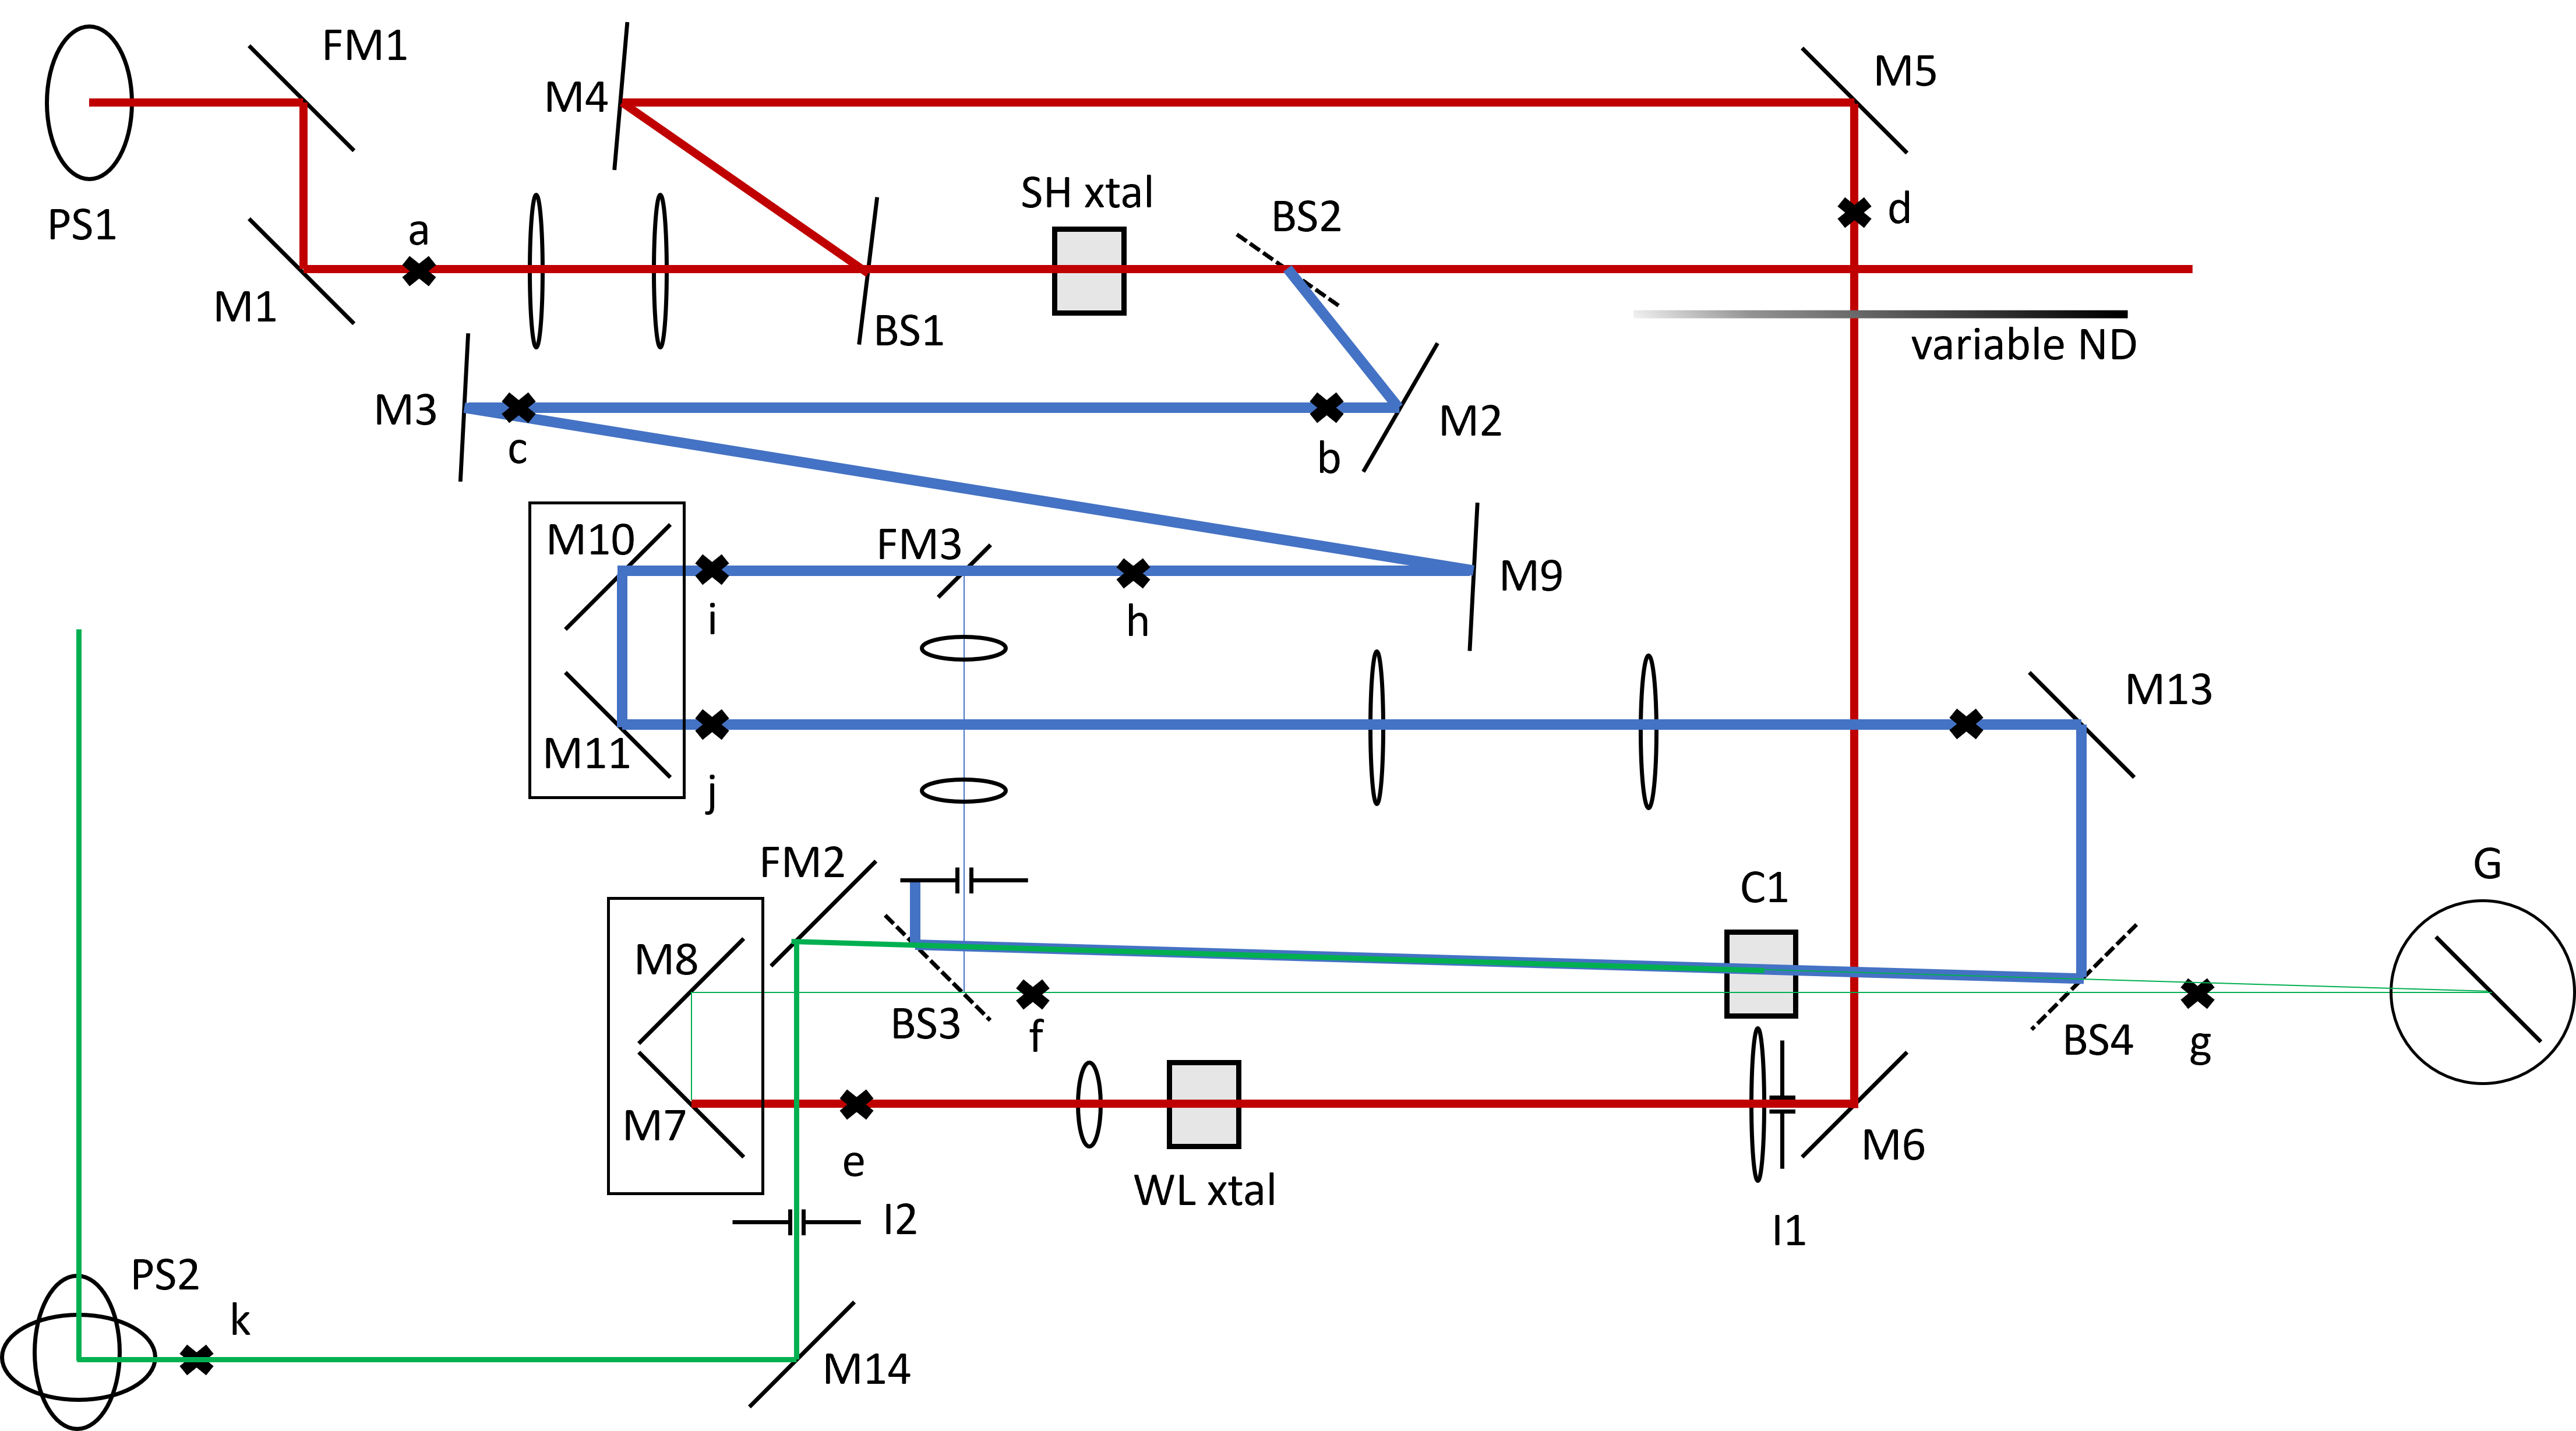
\includegraphics[width=6in]{opa400/images/opa400_schematic}
\caption[OPA 400 Optics]{
	Schematic view of OPA400.
	Input 800 nm light shown in red, doubled 400 nm light shown in blue, parametric output shown in green.
}
\label{opa4:fig:opa_schematic}
\end{figure}

\begin{figure}
	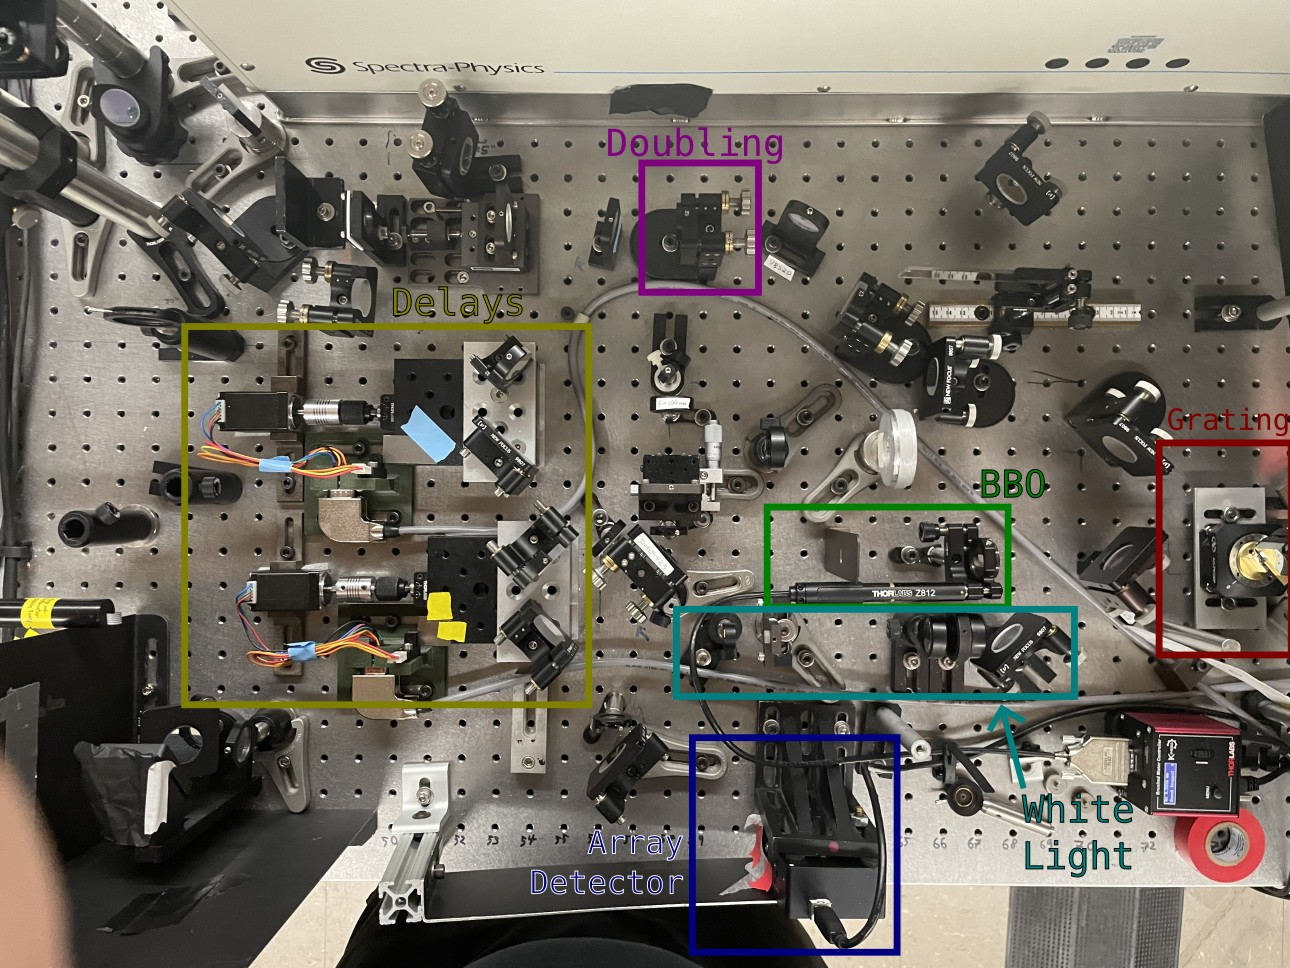
\includegraphics[width=6in]{opa400/images/opa400}
\caption[OPA 400 Optics]{
	Aerial view of OPA400. The 800 nm light enters at the top left and is doubled to 400 nm (purple). 
	A small portion of 800 nm light is used to generate white light (teal).
	The white light and a portion of the 400 nm pump light are combined initially in the BBO (green).
	This creates a broad spectrum output that is bounced off of the grating (red) back to the BBO (green).
	The delays (yellow) ensure that light arrives in the BBO at the same time, which is a requirement for mixing to occur.
	An array detector (blue) allows monitoring of the output visible signal photons.
}
\label{opa4:fig:opa_photo}
\end{figure}

\subsection{Hardware Selection}

The hardware solected follows a ``homebuilt'' approach.
Where possible, namely for the delay stages, standard NEMA stepper motors were used because they are cheap and highly available.
Where precision and/or compactness was a strict requirement, commercially available motors were used.
This includes the Thorlabs Z812\cite{thorlabs_z812} motor for controlling the angle of the BBO Crystal and the Newport CONEX-AGP\cite{newport_conex_agp} rotational mount for the grating.

Creating a complex component such as an OPA is an iterative process, with needs evolving as testing is performed.
For example, initially we opted not to include a grating, relying on phase matching angle alone for selectivity of the signal photon color.
This proved possible, but not as efficient or stable as we desired, so the grating was added as a revision.
The array detector, an Ocean Optics USB2000, is an optional but convenient addition which provides a tighter feedback loop when aligning the OPA.
Additionally, the original design used a Newport stepper motor to control the crystal angle.
The intent was to drive this motor with alternate stepper motor drivers.
This motor did not ultimately work as desired, so it was replaced with the Thorlabs motor and the associated manufacturer provided motor driver.

\section{Stepper Control Box}  % ===================================================================

The control system for this OPA centers around a Raspberry Pi 4\cite{rpi4}.
The stepper motors are driven by Adafruit Stepper Motor HATs\cite{adafruit_stepper_hat}.
These stepper motor drivers come in a convenient form of a circuit board that fits directly on top of the Raspberry Pi.
Each board can support two stepper motors, driven at a voltage provided to a power input that is not shared to the Raspberry Pi itself.
These boards can stack, allowing as many stepper motors as needed to be controlled from the same computer.

On top of the stepper motor driver boards, another hat is used to provide limit switch inputs.
This board is custom designed, containing eight digital inputs which accept 5 Volt input signal and provide a 3.3 Volt signal to the Raspberry Pi General Purpose Input Output (GPIO) pins.
The correspondence between input number as provided by the hat and digital GPIO pin used by the Raspberry Pi is provided in Table \ref{opa4:tab:interrupt_pinout}.
Each input has three pins associated with it: 5 Volts, Ground, and a signal pin.
The signal pin has a pull-up resistor for 5 Volts.
If a simple mechanical switch is used for the input, a nominally open switch between the signal and ground is sufficient.
The 5 Volt line is provided so that sensors such as optical interrupts which require power to operate can be used easily.
Figure \ref{opa4:fig:interrupt_schematic} shows a schematic representation of the schematic for the level conversion and LED indicator for a single input.
This motif is repeated eight times.
Figure \ref{opa4:fig:interrupt_board} shows a rendering of the circuit board itself.

\begin{table}[]                                                                                                     
\begin{tabular}{ll}                                                                                                 
\hline                                                                                                              
Interrupt Number & GPIO Pin   \\ \hline                                                                                        
1   & 17 \\                                                                                               
2   & 22 \\                                                                                               
3   & 5  \\                                                                                               
4   & 6  \\                                                                                               
5   & 13 \\                                                                                               
6   & 26 \\                                                                                               
7   & 23 \\                                                                                               
8   & 24 \\ \hline                                                                                        
\end{tabular}                                                                                                       
        \caption[Interrupt Hat GPIO Pins]{The pin correspondence the interrupt hat.}                         
        \label{opa4:tab:interrupt_pinout}                                                                                        
\end{table}     


\begin{figure}
	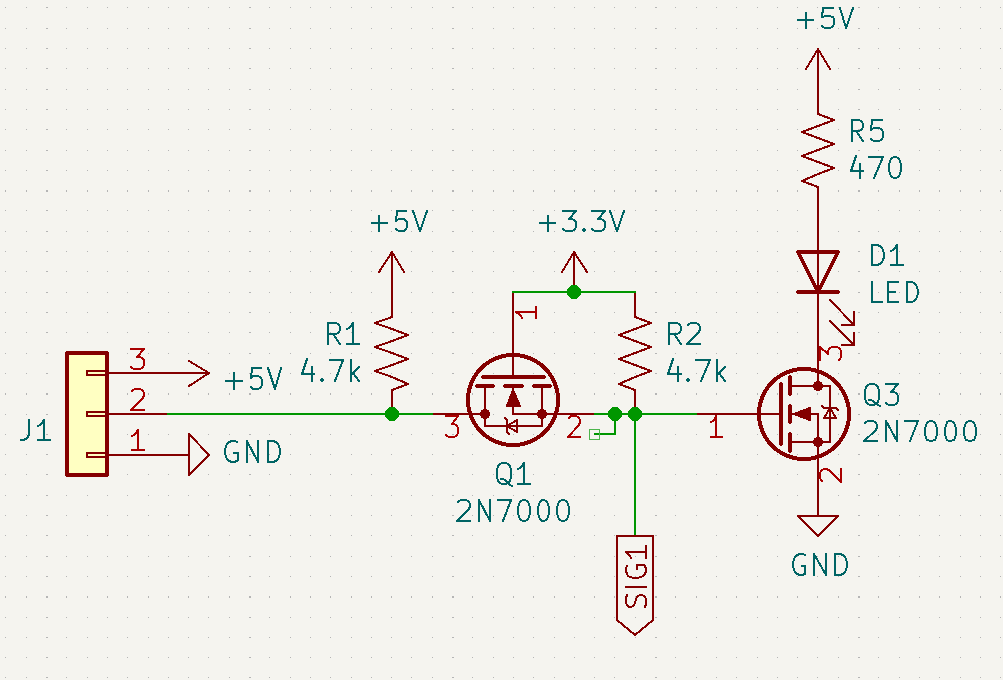
\includegraphics[width=5in]{opa400/images/interrupt_schematic}
\caption[Interrupt Hat Schematic]{
	A schematic view of a single input for the Interrupt Hat.
}
\label{opa4:fig:interrupt_schematic}
\end{figure}


\begin{figure}
	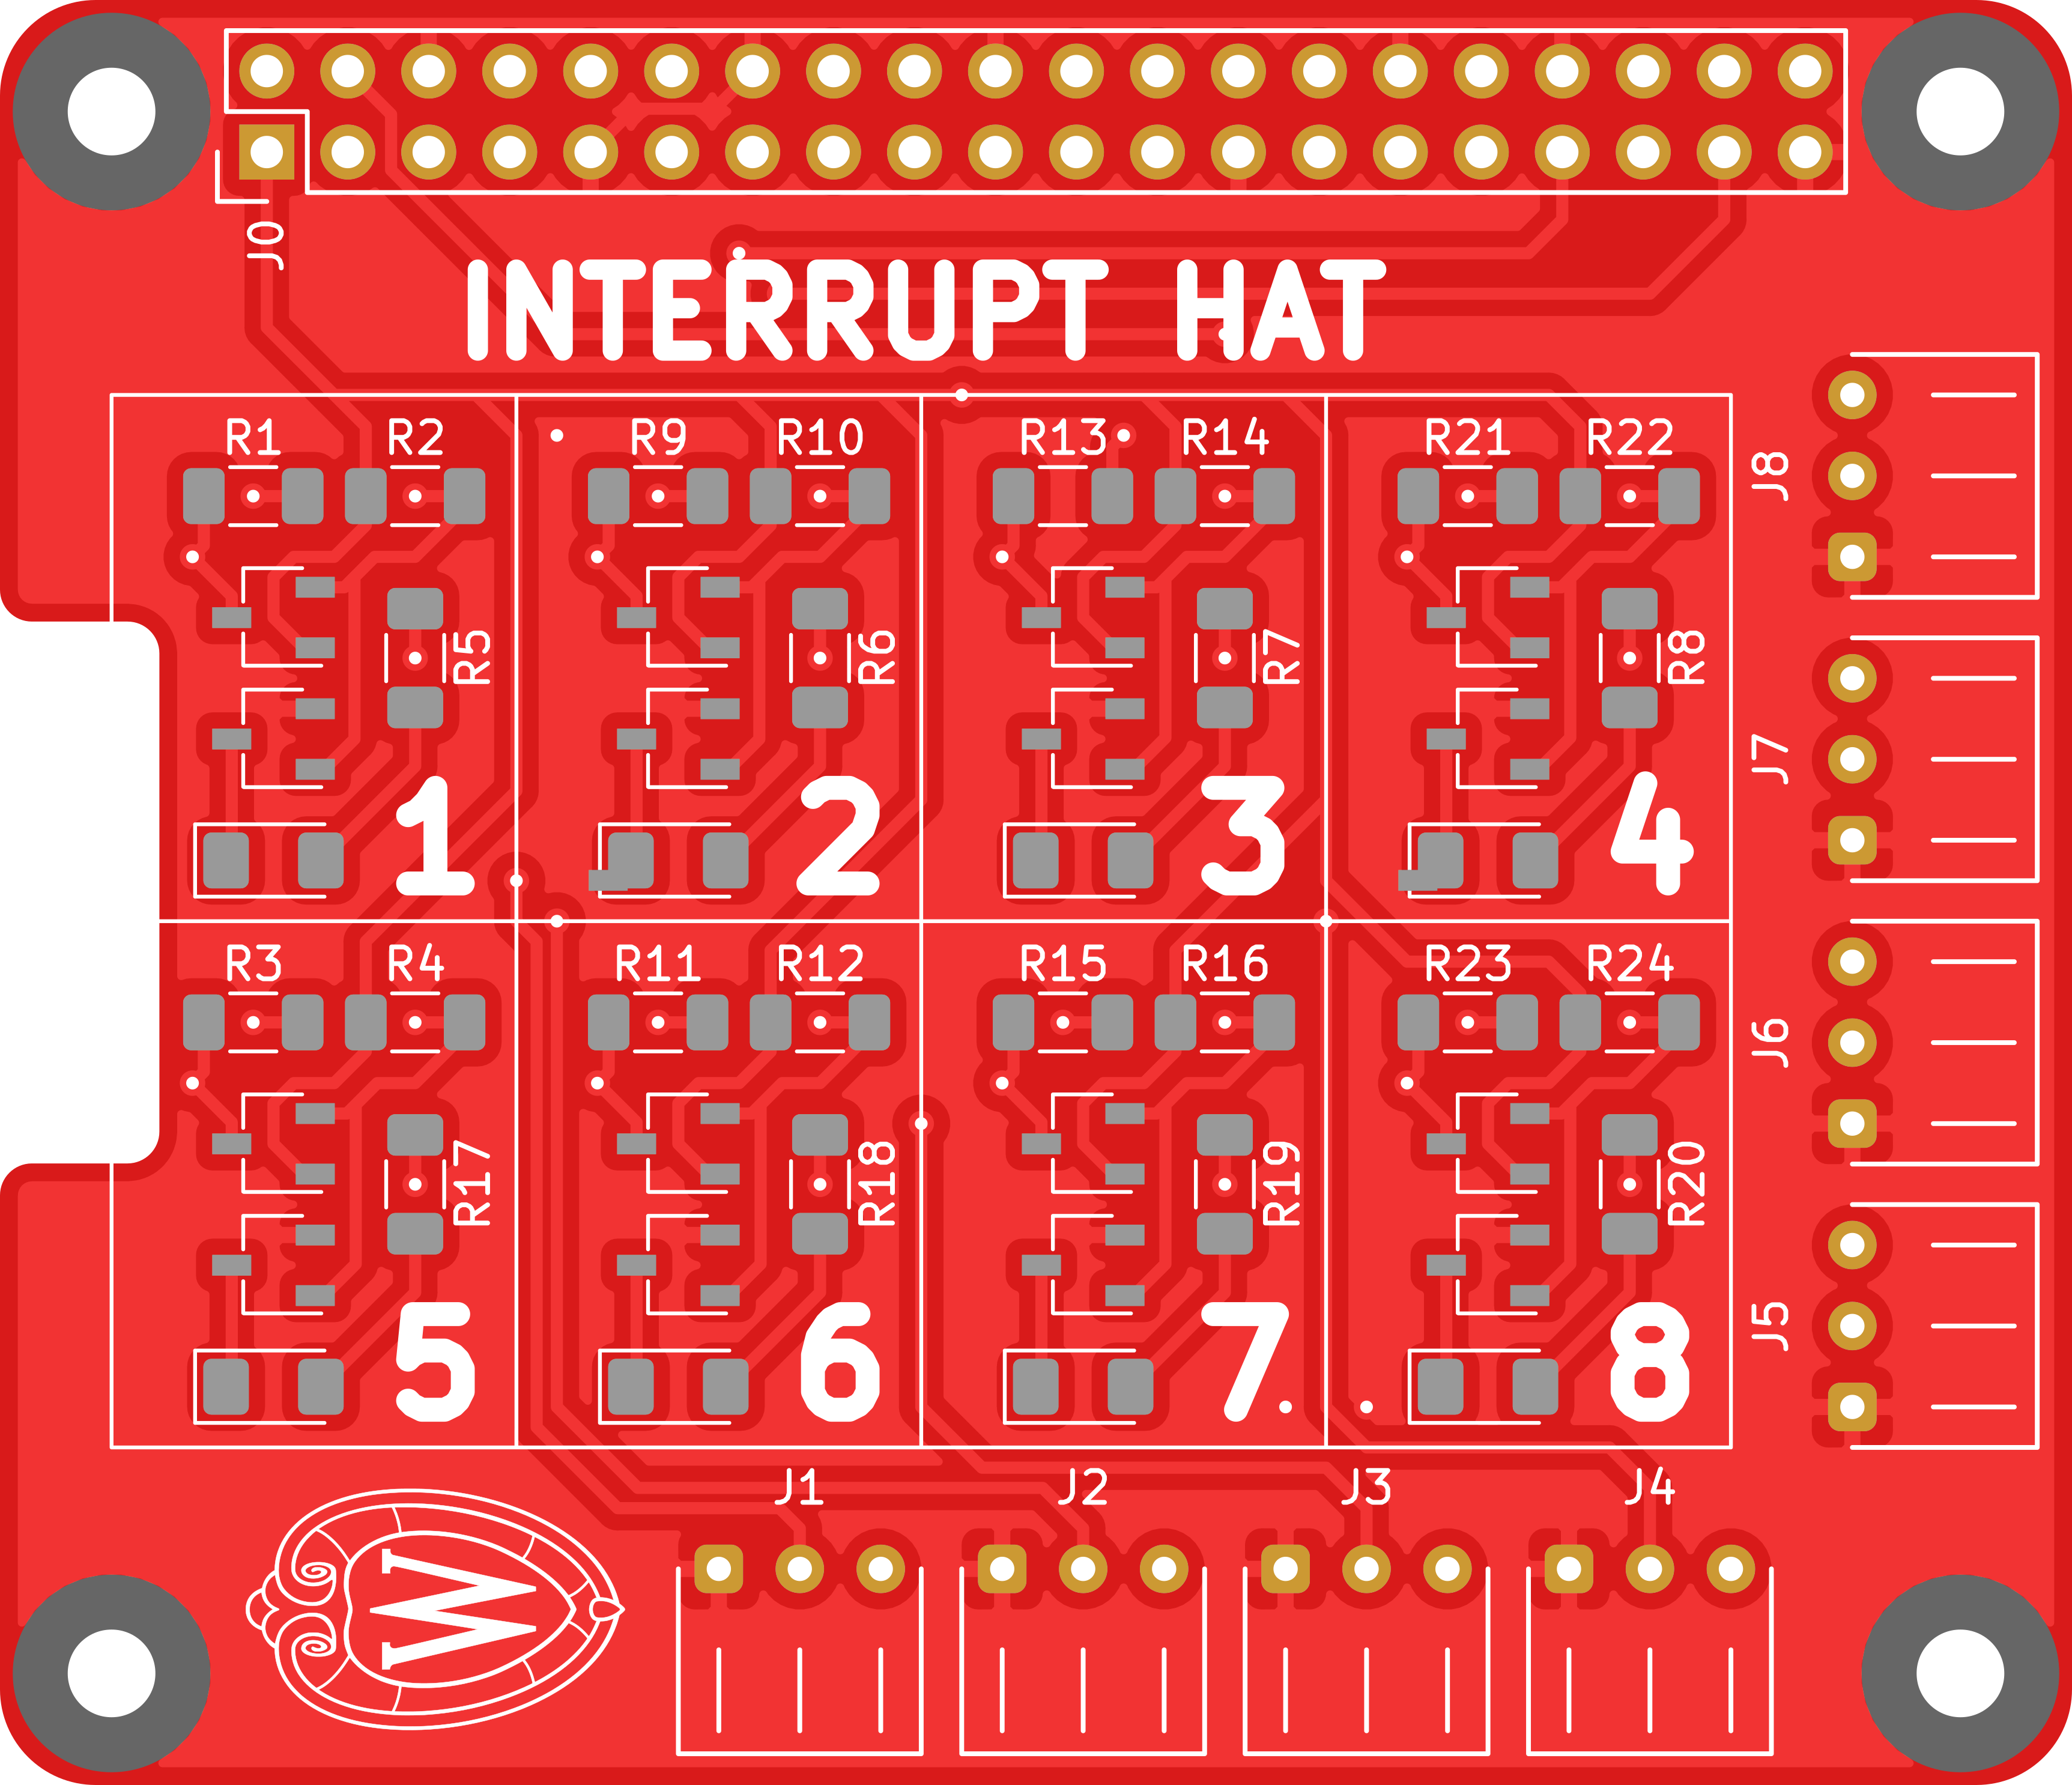
\includegraphics[width=4in]{opa400/images/interrupt_top}
	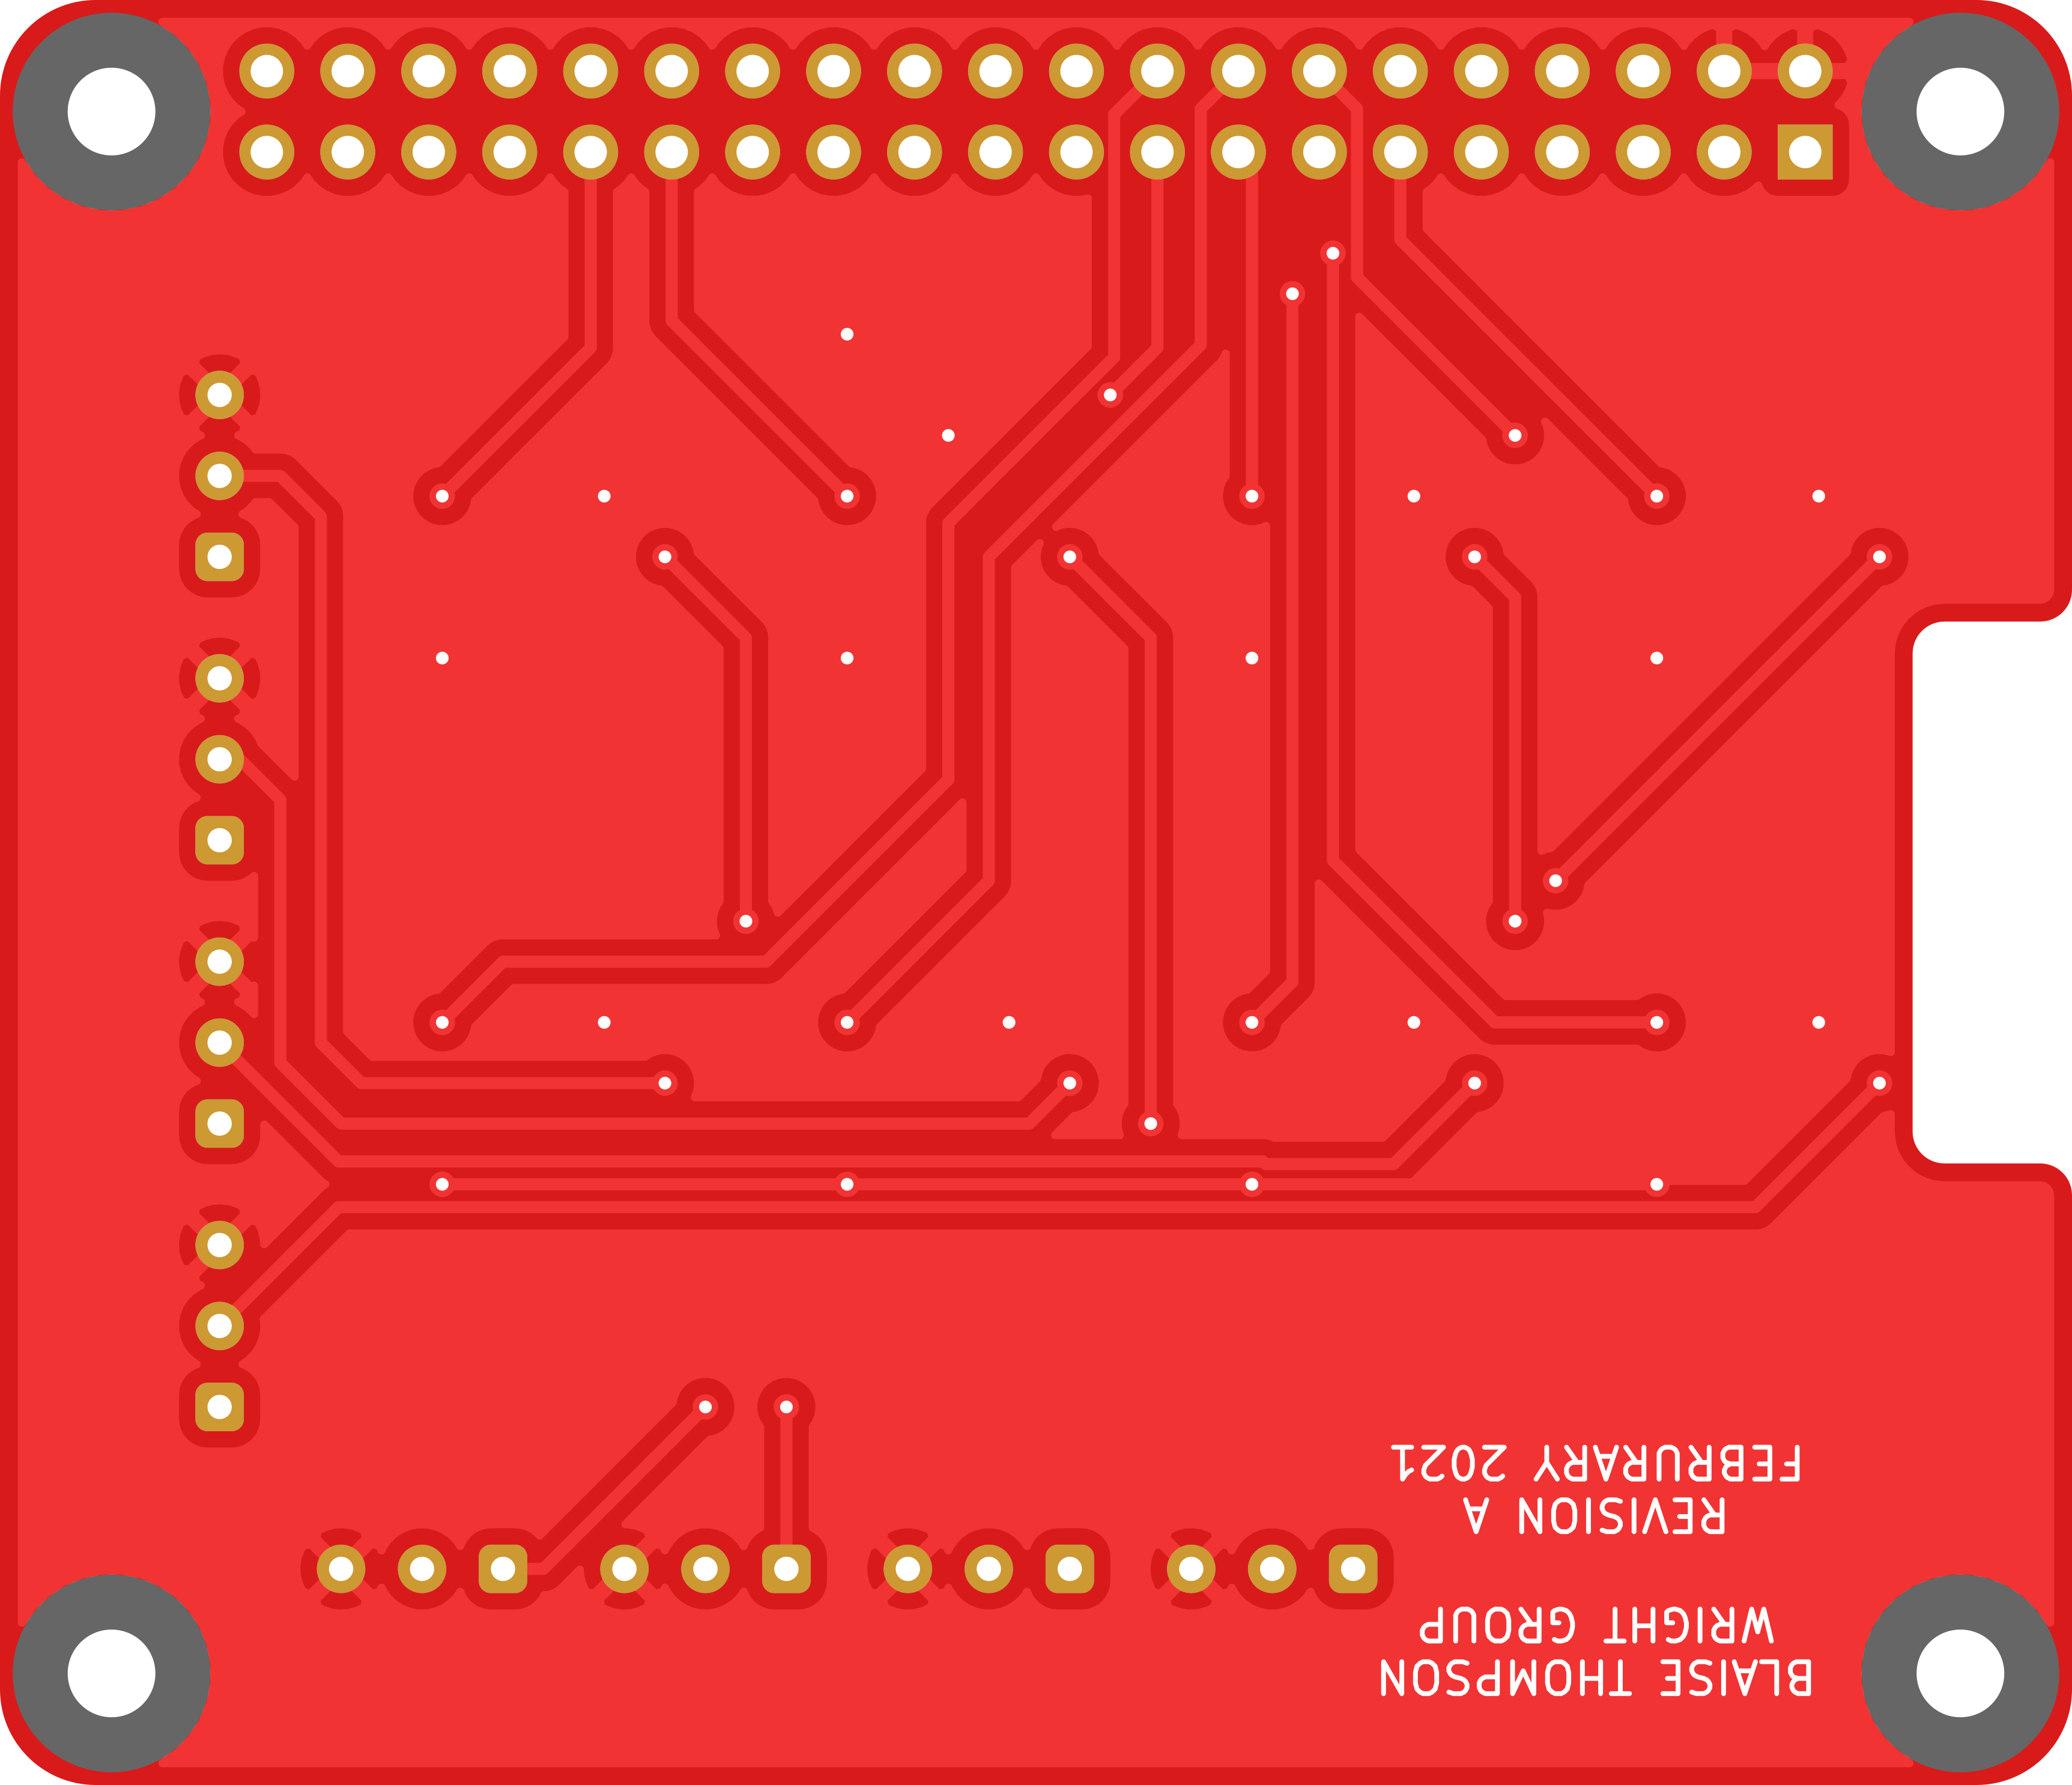
\includegraphics[width=4in]{opa400/images/interrupt_bottom}
\caption[Interrupt Hat Circuit Board]{
Rendering of the interrupt circuit board, top view and bottom view.
Rendering performed using tracespace\cite{tracespace}.
}
\label{opa4:fig:interrupt_board}
\end{figure}

The stepper control box is designed to work with the Mean Well RS-15 series of DC power supplies\cite{meanwell_rs15}.
Each hat level (two steppers) can accept an independent voltage level, so stepper motors with differing specifications can be used and controlled by the same system.
The box is designed so that three power supplies can be installed as needed.
One of the power supplies should be a 5 Volt power supply so that the Raspberry Pi itself can be powered from the same source.

The box is constructed of metal base with mounting holes drilled for the power supplies and the Raspberry Pi assembly.
At the corners of the base, 15 mm aluminum extrusion posts provide support for the panels.
The side panels and top are clear acrylic cut to size to slot in to the aluminum extrusion.
The top is secured with screws, with tapped 3 mm screw holes in the center of the posts.
This allows visual access to the LED indicators of the Interrupt Hat.
The front and rear panels are 3D printed plastic, with mounting for connectors.
The rear panel has AC power input and a power switch.
The front panel has a cut out for access to the Raspberry Pi USB and Ethernet ports as well as connectors for the stepper motors.
The pinout for the Wright Group's standard DE-9 D-subminiature stepper motor port is provided in Table \ref{opa4:tab:de9}.
Figure \ref{opa4:fig:control_box_photo} shows a photograph of the completed control box.

\begin{table}[]
\begin{tabular}{ll}
\hline
Pin & Connection   \\ \hline
1   & NC           \\
2   & Limit Signal \\
3   & +5 V         \\
4   & GND          \\
5   & NC           \\
6   & B2           \\
7   & B1           \\
8   & A1           \\
9   & A2           \\ \hline
\end{tabular}
	\caption[Stepper Motor DE9 Pinout]{The pinout for the stepper motor DE9 connector.}
	\label{opa4:tab:de9}
\end{table}

\begin{figure}
	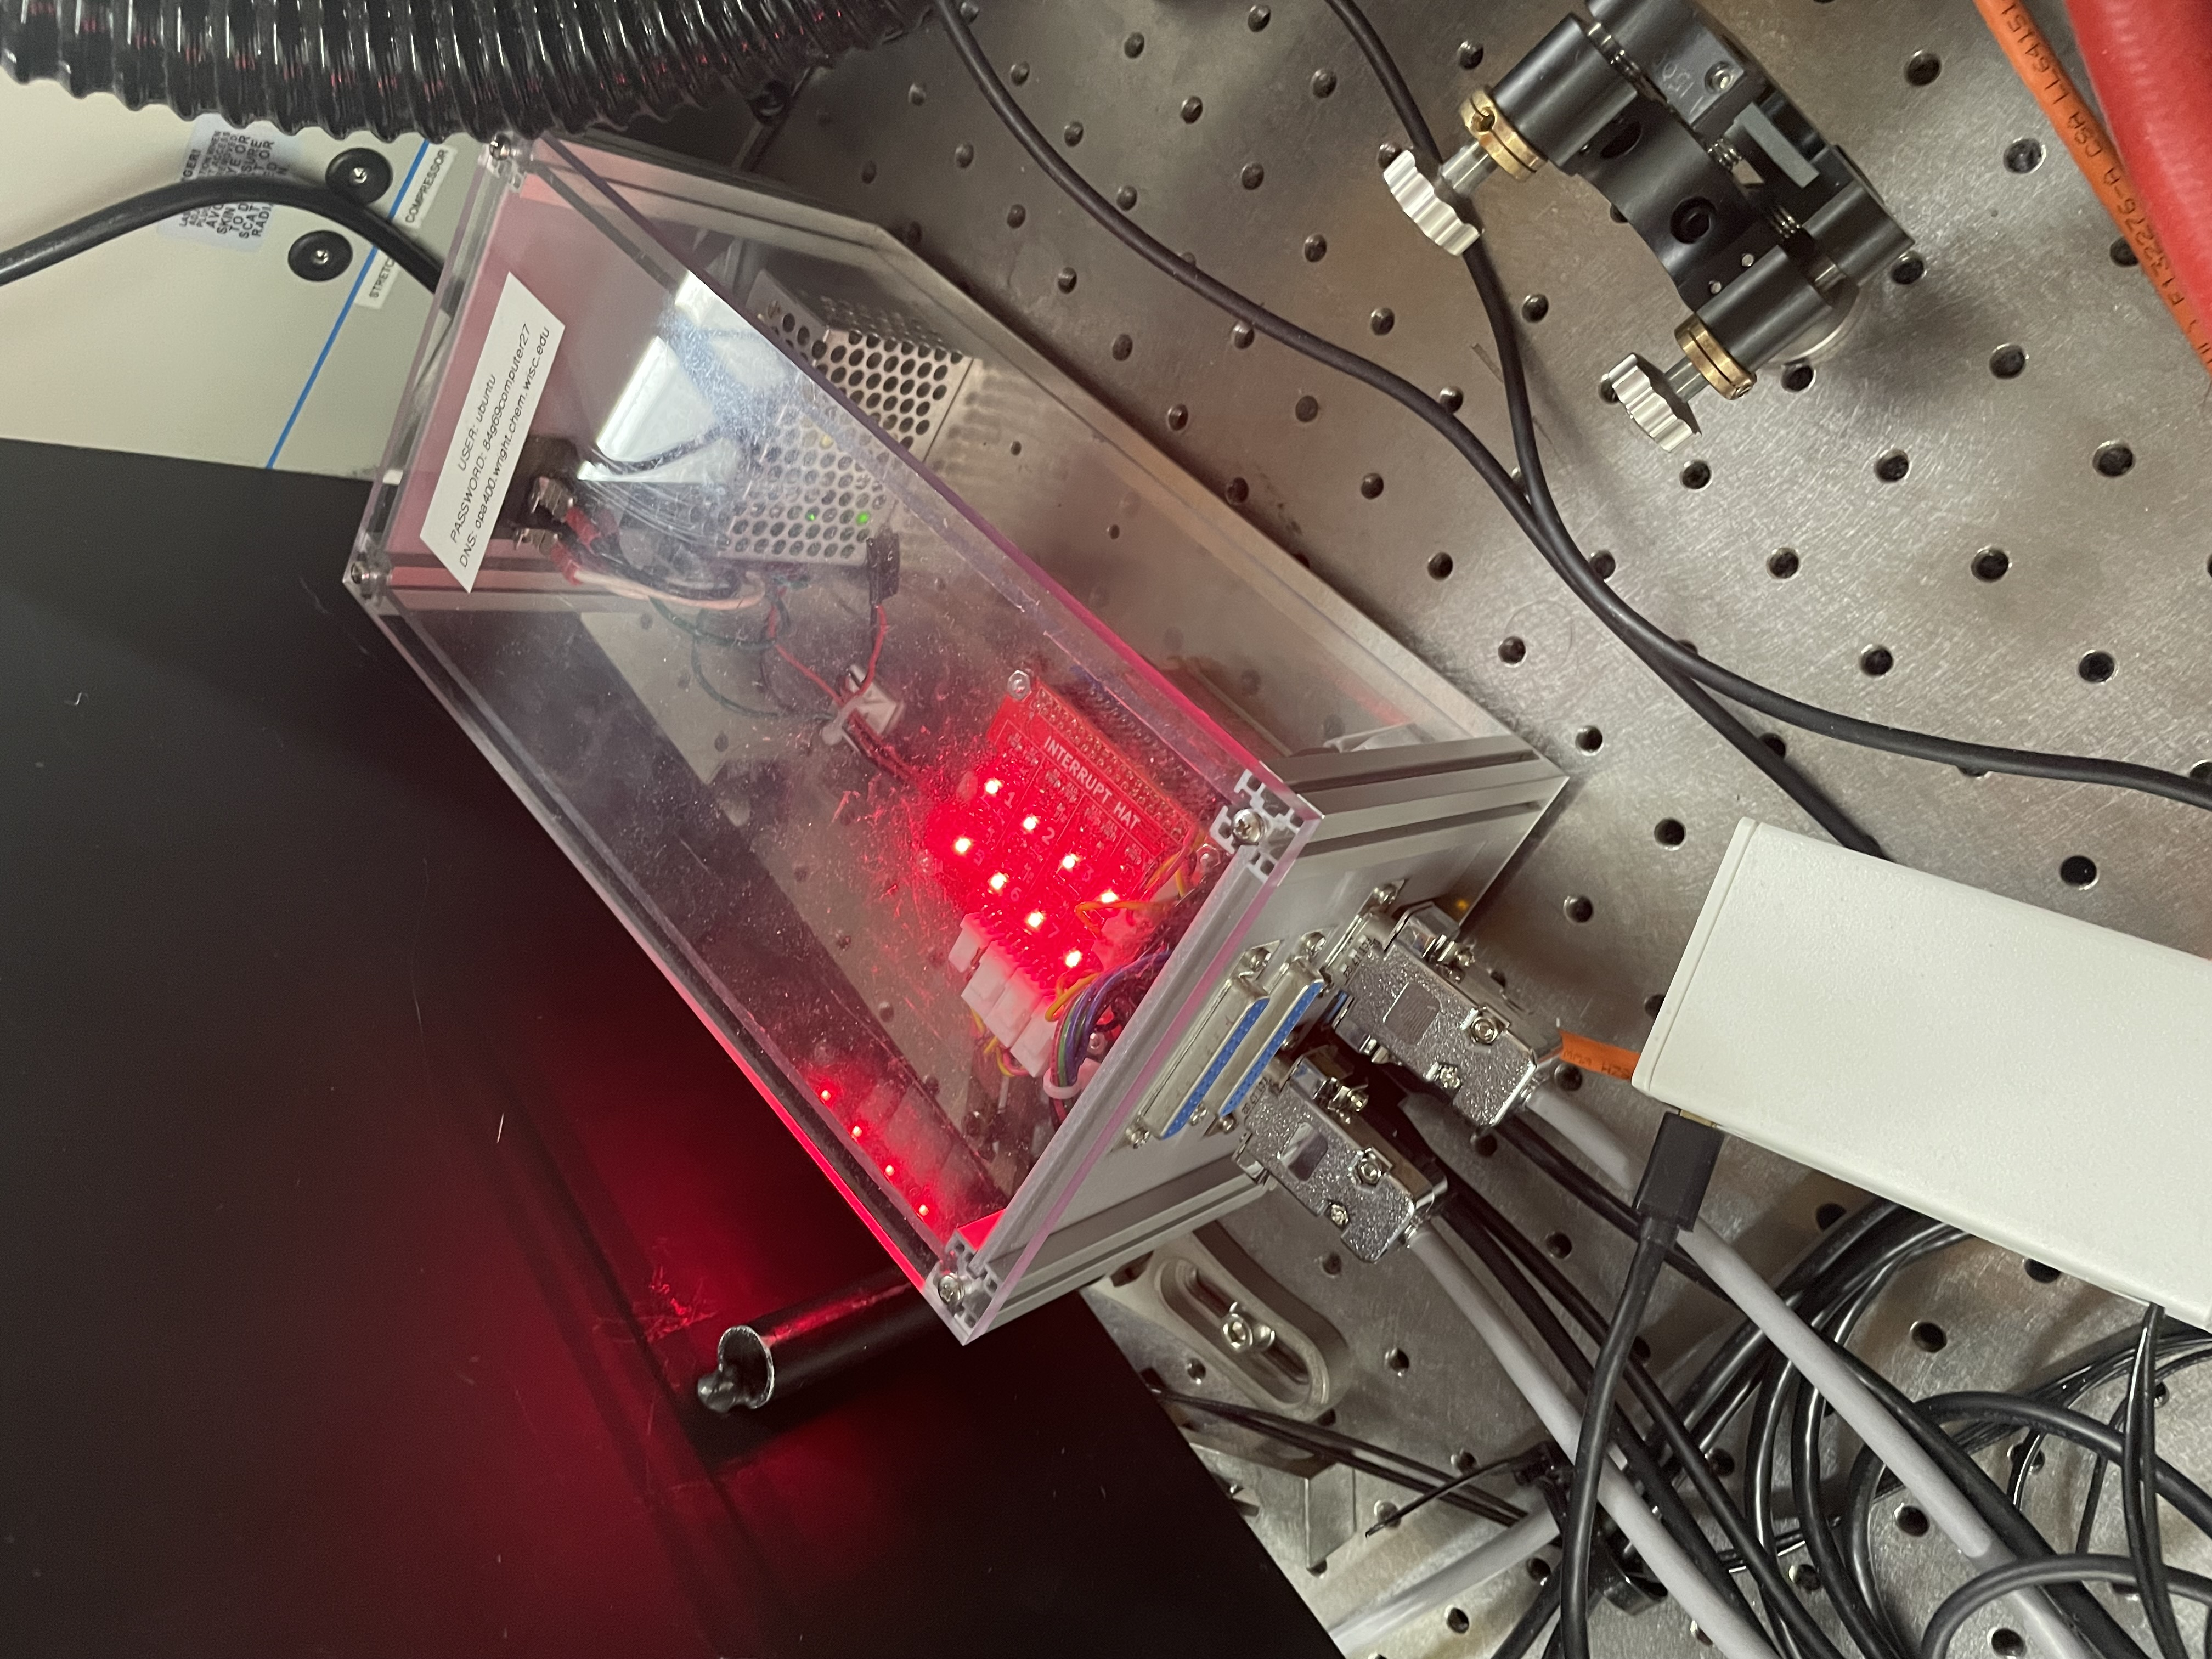
\includegraphics[width=5in]{opa400/images/opa400_control_box}
\caption[Stepper Control Box]{
Photograph of the stepper control box.
}
\label{opa4:fig:control_box_photo}
\end{figure}


\section{Delay stages}  % ===================================================================

The delay stages themselves have custom components designed for this application.
A 3D printed part provides a mount for a connector and the optical interrupt which is used for homing the motor.
A small piece of sheet metal is the flag which interrupts the optical interrupt.
The delay mechanism itself is a simple manual translation stage purchased from Thorlabs\cite{thorlabs_pt1b}.
This stage has a fine lead screw which provides the necessary precision to properly overlap the picosecond light pulses.
Below the stage, a machined aluminum block raises the stage to a height where the motor can directly drive the lead screw.
There is an additional adapter plate on top of the translation stage which provides a low profile mount for two mirrors at 90 degrees from each other, forming a planar retroreflector.
The custom machined parts in this system are important because space, particularly vertical space, is limited to have the mirrors in the desired position.
These parts were machined out of aluminum rather than 3D printed with consideration of the thermal expansion and rigidity of the parts which are directly supporting the optics.

The motors are coupled to the stage using a small aluminum rod machined to size and epoxied in place and a spring coupler which was purchased as a part for a 3D printer.
The motors themselves are mounted using two L-brackets pinching the motor.
Originally, the design included mounting the motor to the 3D printed part which also houses the connector and interrupt.
This proved problematic, as the forces exerted on the motor in the designed configuration meant it was unable to turn the stage.
Aligning the motor so that it can turn the stage is not difficult, but required more flexibility than a single mounting point of the 3D printed part.


\clearpage

\section{Software}  % ===================================================================

To control OPA400, a series of \yaq{} daemons were implemented.
Two of the motors were commercial products, the Thorlabs motor for the BBO crystal and the Newport motor for the grating.
These two had extant daemons already implemented prior to their use for OPA400\cite{yaqd-thorlabs}\cite{yaqd-newport}.
The Newport motor was already in use in other experimental setups, and had been written with the particular hardware that ended up installed in OPA400.
The Thorlabs motor was purchased specifically for this project, but uses a common protocol with other similar motors.
The daemon was already implemented, though it was tested specifically with the controller prior to installation.
These daemons can run directly on the Raspberry Pi, which makes for simpler cable management.

In addition to the previously created daemons, a new daemon was made to control the Adafruit stepper motor drivers.
This daemon uses two python libraries provided by Adafruit, the CircuitPython MotorKit\cite{adafruit-circuitpython-motorkit} and CircuitPython Motor\cite{adafruit-circuitpython-motor} libraries, as well as one library for interacting with the Raspberry Pi GPIO pins, GPIO Zero\cite{gpiozero}.
The first two are used to control the stepper motor, instructing each individual step.
The latter is used to read the state of the optical interrupt.
The daemon, implemented in about 100 lines of Python code, allows users to interact with the delay stages as they would with a daemon implemented for a commercial product.
Originally, this daemon was going to use another daemon for reading the interrupt state, but that was abandoned because of timing considerations and the fact that a daemon built for a Raspberry Pi hat is already a well constrained environment.
These daemons must be run directly on the Raspberry Pi, as they need direct hardware access to the GPIO pins.

Once each individual motor has an appropriate daemon implemented, the motors can be included in an Attune Instrument, just like other OPA models.
This Attune Instrument has its own daemon that can run on main instrument machine, which allows for easy access to update and read the Attune Instrument history.

When starting a new Attune Arrangement (or in this case a new Instrument altogether) a good initial strategy is to manually find appropriate motor positions for a small number of points.
Approximately five points, including points near to both ends of the expected usable range, is usually good enough to allow a general sense of the curvature of each Tune.
This rough tuning curve can be scaled up to more points (often around 20 points, though the degree of curvature and range will vary how many points are required for satisfactory interpolation) using \texttt{attune.map\_ind\_points}.
This upscaled Tune will not be fully accurate, but will usually be close enough that the standard tuning procedures can capture the offsets.

The standard tuning procedure for OPA400 is as follows.
First, a careful alignment of the optics, following standard operating procedures to align to apertures and obtain single color output.
Second a \texttt{run\_intensity} for the pre-amp delay (D1, the white light line) with the grating at normal incidence.
Third, a \texttt{run\_tune\_test} of the pre-amp color, using the array detector.
Fourth, a \texttt{run\_intensity} for the grating positions, detecting first pass amplification through an aperture.Finally, the second pass delay (D2, the delay for 400 nm light) is offset appropriately.
In theory, this delay needs to compensate for some additional spectral delay inside of the OPA.
In practice, a static offset is usually good enough for the whole range of colors.

\clearpage
